% =====================================================================
%  Dynamic Scientific Storytelling -- Midterm Project Report
%  "Dimples, Drag, and Backspin"  --  Michael Niemeyer Jr.
%  Compile with pdfLaTeX (Overleaf default). Upload the whole folder:
%  main.tex, numbers.tex, checks_table.tex, validation_table.tex, figures/.
%  numbers.tex and the two tables are generated by prep/report_numbers.py.
% =====================================================================
\documentclass[11pt]{article}
\usepackage[margin=1in]{geometry}
\usepackage[T1]{fontenc}
\usepackage{lmodern}
\usepackage{microtype}
\usepackage{amsmath,amssymb}
\usepackage{siunitx}
\usepackage{booktabs,tabularx,array,longtable}
\usepackage{enumitem}
\usepackage{float}
\usepackage{graphicx}
\usepackage{caption}
\usepackage{xcolor}
\usepackage{listings}
\usepackage{textcomp}
\usepackage[colorlinks=true,linkcolor=blue!50!black,urlcolor=blue!50!black,citecolor=blue!50!black]{hyperref}

% generated by prep/report_numbers.py -- do not edit
\newcommand{\CalCdOne}{0.200}
\newcommand{\CalClOne}{0.530}
\newcommand{\CalCarry}{278.7}
\newcommand{\CalErrYd}{-3.3}
\newcommand{\CalErrPct}{-1.2}
\newcommand{\CalN}{153}
\newcommand{\RawDrvCarry}{253.0}
\newcommand{\RawDrvErr}{-29.0}
\newcommand{\RawLDrvErr}{-8.9}
\newcommand{\MaeCalL}{23.0}
\newcommand{\MaeApexCalL}{4.3}
\newcommand{\MaeLandCalL}{4.8}
\newcommand{\MaeCalP}{20.3}
\newcommand{\MaeApexCalP}{6.8}
\newcommand{\MaeLandCalP}{6.2}
\newcommand{\MaeRawL}{11.0}
\newcommand{\MaeApexRawL}{2.7}
\newcommand{\MaeLandRawL}{4.0}
\newcommand{\MaeRawP}{8.2}
\newcommand{\MaeApexRawP}{3.5}
\newcommand{\MaeLandRawP}{5.6}
\newcommand{\HeldRaw}{8.6}
\newcommand{\HeldCal}{22.4}
\newcommand{\IronLandErr}{-5.1}
\newcommand{\IronOutside}{88}
\newcommand{\VacDrv}{231}
\newcommand{\VacDrvFortyFive}{651}
\newcommand{\ModDrvFortyFive}{184}
\newcommand{\HeadLoss}{23}
\newcommand{\TailGain}{20}
\newcommand{\DenverGain}{22}
\newcommand{\DenverRho}{1.047}
\newcommand{\SmoothCarry}{171}
\newcommand{\FadeLat}{18.5}
\newcommand{\DragOnly}{134}
\newcommand{\OptCarry}{259}
\newcommand{\OptTheta}{17.0}
\newcommand{\OptRpm}{2500}
\newcommand{\NSpeeds}{20}
\newcommand{\NGridRuns}{148{,}840}
\newcommand{\NRuns}{138}
\newcommand{\NTraj}{55{,}611}
\newcommand{\NChecks}{11}
\newcommand{\NPass}{11}
\newcommand{\WSzero}{0.0744}
\newcommand{\WCDzero}{0.3065}
\newcommand{\WCLzero}{0.1910}
\newcommand{\WFD}{1.569}
\newcommand{\WFL}{0.977}
\newcommand{\Wweight}{0.451}
\newcommand{\WRe}{220{,}761}

% Generated tables are read with the primitive \@@input so they work inside tabular/longtable.
\makeatletter\newcommand{\inputrows}[1]{\@@input #1 }\makeatother
\sisetup{per-mode=symbol}
\setlist{itemsep=2pt,topsep=3pt}
\captionsetup{font=small,labelfont=bf}
\graphicspath{{figures/}}
\setlength{\LTcapwidth}{\textwidth}

% Items the author must fill in or confirm before submitting (shown in orange).
\newcommand{\todo}[1]{\textcolor{orange!85!black}{#1}}

\lstset{basicstyle=\ttfamily\scriptsize,breaklines=true,frame=single,framerule=0.3pt,
        rulecolor=\color{black!30},backgroundcolor=\color{black!3},
        keywordstyle=\color{blue!60!black}\bfseries,commentstyle=\color{green!40!black},
        columns=fullflexible,showstringspaces=false}

\title{\textbf{Dimples, Drag, and Backspin:}\\
       \large An Explorable Story of Why a Golf Ball Flies the Way It Does\\[4pt]
       \normalsize Dynamic Scientific Storytelling --- Midterm Project}
\author{Michael Niemeyer Jr.\\
        Department of Computer Science and Technology, Kean University}
\date{October 2026}

\begin{document}
\maketitle

\begin{center}
\small
\begin{tabular}{@{}ll@{}}
\textbf{Working visualization} & \todo{\url{https://obi2.kean.edu/~niemeymi/golf/}} \\
\textbf{Source code and data}  & \todo{GitHub repository URL} (also submitted as \texttt{golf-story.zip}) \\
\textbf{Launch instructions}   & Section~\ref{sec:launch} and \texttt{README.md} \\
\end{tabular}
\end{center}

% =====================================================================
\begin{abstract}
\noindent
A PGA Tour driver leaves the clubface at \SI{171}{mph} with \SI{2545}{rpm} of backspin and carries
\SI{282}{yd} on average, yet the vacuum projectile formula taught in introductory physics predicts
\VacDrv{}~yd at the same launch angle and \VacDrvFortyFive{}~yd at \ang{45}. This project implements
the approved proposal as a working, seven-view explorable story that explains the mechanism behind
real golf-ball flight: drag, which the dimples reduce, and Magnus lift, which backspin creates.
The story is driven by an explicitly labeled scientific simulation (a three-dimensional point-mass
model integrated with fourth-order Runge--Kutta, using the aerodynamic model of Smits and Smith,
1994) and is validated against 23 measured club averages from TrackMan's 2023 PGA and LPGA Tour
tables. The model reproduces the PGA driver's apex and landing angle closely but under-predicts its
carry by \RawDrvErr{}~yd with the published wind-tunnel constants; calibrating two constants inside
the paper's own ranges fixes the driver (\CalErrYd{}~yd) but makes the 22 held-out clubs worse (mean
absolute error \HeldRaw{} to \HeldCal{}~yd). The story shows both results rather than hiding either.
All \NChecks{} planned numerical and boundary checks pass, after one boundary check exposed and
helped fix a real integration bug.
\end{abstract}

% =====================================================================
\section{Introduction}

\paragraph{Guiding question.} \emph{Why does a spinning, dimpled golf ball fly so differently from
the ideal projectile of introductory physics, and which launch conditions (speed, angle, spin)
produce the longest carry?}

\paragraph{Audience.} First- and second-year STEM undergraduates who know constant-acceleration
kinematics but have not studied fluid dynamics, and curious golfers with no physics background.
Every golf term (carry, apex, launch angle, backspin) is defined on first use and every quantity is
shown with units; a global toggle switches between golf units (yd, mph, rpm, ft) and SI.

\paragraph{Objectives.} After using the story, a reader should be able to:
(O1) explain why the vacuum model both under- and over-predicts real carry depending on launch
angle; (O2) name the three forces in flight and how each changes; (O3) explain how the spin ratio
$S=r\omega/u$ controls lift and drag; (O4) use the explorer and the launch-window map to find a
near-optimal launch and explain the angle--spin trade-off; (O5) predict the effect of wind and
altitude; and (O6) say how well the model matches measured data and where it should not be trusted.
Table~\ref{tab:objectives} maps each objective to the view that serves it.

% =====================================================================
\section{Related Work}

\textbf{The LLM Story}~\cite{llmstory} (the course exemplar) builds understanding through a
sequence of linked, dynamic views of a transformer. This project borrows its structure, a staged
narrative in which each view answers one question, and applies it to a physical mechanism. Nothing
in the code, visual design, or narrative is copied from it.
\textbf{Explorable explanations}~\cite{victor2011} argue that readers learn a model best when they
can change its assumptions and watch the consequences; Views~4--6 follow this idea directly.
\textbf{PhET's Projectile Motion}~\cite{phet} varies angle and speed with an on/off air-resistance
toggle but has no spin and no lift; the Magnus effect is the core of this project.
On the physics side, Bearman and Harvey~\cite{bearman1976} measured golf-ball lift and drag in a
wind tunnel; Smits and Smith~\cite{smits1994} built on those measurements, added spin-decay
measurements, and proposed the driver-only aerodynamic model used here; Penner~\cite{penner2003}
reviews the physics of golf; and Choi, Jeon, and Choi~\cite{choi2006} explain how dimples trigger a
turbulent boundary layer that delays separation. TrackMan publishes tour-average launch data
\cite{trackman2023} but presents numbers, not mechanism. Visual-design choices follow
Munzner~\cite{munzner2014}: position before color, sequential color for ordered magnitude, and 3D
only where the phenomenon is three-dimensional.

% =====================================================================
\section{Methodology and Workflow}

\subsection{Changes from the approved proposal}\label{sec:changes}

The project follows the proposal's question, audience, seven-view storyboard, equations, data
sources, checks, and interaction plan. Table~\ref{tab:changes} lists every deliberate change and
why it was made.

\paragraph{Instructor feedback on the proposal.} \todo{Summarize the feedback you received on the
proposal here (one to three sentences per point) and, for each point, say which change below or
which part of the implementation addresses it. If no written feedback was received, say so.}

\begin{longtable}{@{}p{0.31\textwidth}p{0.64\textwidth}@{}}
\caption{Changes from the approved proposal, with reasons.}\label{tab:changes}\\
\toprule
Proposal plan & Implemented, and why \\
\midrule
\endfirsthead
\toprule Proposal plan & Implemented, and why \\ \midrule \endhead
Plotly.js for 2D charts, Three.js for View~6. &
Plain JavaScript and HTML Canvas with no libraries, including a hand-written perspective camera for
View~6. The page then opens offline from a single folder, so the live demo cannot fail on a CDN or
network, and every drawing step is code I can explain in the presentation. \\
Coefficient model of Eq.~3 (revised proposal). & Implemented exactly, including the Reynolds-number
sine term and the spin-decay law $\dot\omega\,r^2/u^2=-R_1S$, with all seven published constants. \\
View~3 ``Show source points'' overlay of digitized wind-tunnel data. & Dropped. Digitizing the
scanned figures in~\cite{smits1994} could not be done accurately enough to present as data.
Replaced by the drag curve drawn at three Reynolds numbers plus a shaded band showing the range the
fit was made for, which shows the same uncertainty honestly. \\
View~5 grids ``for several fixed $v_0$''. & One $61\times61$ grid at each of the \NSpeeds{} distinct
measured ball speeds, for both coefficient sets (\NGridRuns{} simulated shots). Measured clubs then
sit exactly on the map for their own speed. The color scale covers the top \SI{60}{yd} of each map,
because the full range left almost every cell the same dark color; the legend says so. \\
View~7 hollow marker = ``incomplete reference row''. & The real data gap is a whole missing row
(LPGA 3-iron), which cannot be plotted. It is listed in the legend and table instead, and hollow
markers now mean ``more than half of the flight is outside the model's fitted range''. \\
Binary ``outside model validity'' warning. & A graded badge giving the percentage of flight time
outside the fitted range, because almost every shot leaves the range briefly. \\
Calibration as a one-off step. & A global coefficient-set selector (wind-tunnel vs.\ calibrated)
that every view uses, because calibration turned out to help one club and hurt the rest. \\
Equal-aspect side views throughout. & Kept for Views~1 (toggle), 2 and the View~7 scatter. The
View~6 insets use independent axis scales (labeled), because a straight drive drawn at true
lateral scale is a single flat line. \\
Python/NumPy integrator ``twin''. & Vectorized so it integrates thousands of shots at once; the
View~5 grids take minutes instead of hours. \\
JSON loaded by \texttt{fetch}. & JSON packed into \texttt{data/bundle.js} so \texttt{index.html}
opens from disk without a web server. \\
\bottomrule
\end{longtable}

\subsection{Data and model}

The project combines two sources, labeled \textsc{Measured} and \textsc{Model} everywhere in the
interface and drawn in two fixed colors (orange and blue).

\paragraph{Measured data.} TrackMan's 2023 PGA Tour and LPGA Tour averages~\cite{trackman2023}: 12
clubs per tour, with club speed, attack angle, ball speed, smash factor, launch angle, spin rate,
maximum height, landing angle, and carry (yards and meters). I transcribed both tables by hand into
\nolinkurl{data/trackman_2023_raw.csv}. The LPGA table has no 3-iron; that row is kept with empty
fields and \texttt{complete = 0}. TrackMan's own meter columns served as a transcription check: every
yard value converts to the published meter value within the combined rounding limit
($0.5\,\text{yd}\times0.9144+0.5\,\text{m}=0.957$\,m; largest gap 0.89\,m, PGA 4-iron).

\paragraph{Scientific simulation.} A point-mass, three-dimensional model of a spinning sphere
($m=\SI{45.93}{g}$, $D=\SI{42.67}{mm}$). With $x$ downrange, $y$ to the left and $z$ up, wind
$\mathbf w$, and relative velocity $\mathbf u=\mathbf v-\mathbf w$, $u=\lVert\mathbf u\rVert$:
\begin{equation}
m\dot{\mathbf v} = -mg\,\hat{\mathbf z} - \tfrac12\rho A\,C_D\,u\,\mathbf u
 + \tfrac12\rho A\,C_L\,u^2\,\frac{\hat{\boldsymbol\omega}\times\hat{\mathbf u}}{\lVert\hat{\boldsymbol\omega}\times\hat{\mathbf u}\rVert},
\qquad S=\frac{r\omega}{u},\qquad \mathrm{Re}=\frac{\rho u D}{\mu},
\end{equation}
\begin{equation}
C_D = C_{d1}+C_{d2}S+C_{d3}\sin\!\left\{\frac{\pi(\mathrm{Re}-A_1)}{A_2}\right\},\qquad
C_L = C_{l1}S^{0.4},\qquad \frac{d\omega}{dt}\frac{r^2}{u^2}=-R_1S,
\end{equation}
with Smits and Smith's constants $C_{d1}=0.24$, $C_{d2}=0.18$, $C_{d3}=0.06$, $C_{l1}=0.54$,
$R_1=0.00002$, $A_1=\num{90000}$, $A_2=\num{200000}$~\cite{smits1994}, $\mu=\SI{1.81e-5}{Pa.s}$, and air
density from the U.S.\ Standard Atmosphere troposphere model~\cite{ussa1976},
$\rho(h)=\rho_0(1-Lh/T_0)^{gM/(RL)-1}$ with $\rho_0=\SI{1.225}{kg/m^3}$. The spin axis is
$\hat{\boldsymbol\omega}=(0,-\cos\alpha,-\sin\alpha)$, so pure backspin gives upward lift and a
positive tilt $\alpha$ curves the ball to the right (a fade). The state
$(x,y,z,v_x,v_y,v_z,\omega)$ is integrated with RK4 at $\Delta t=\SI{1}{ms}$; landing is found by
linear interpolation to $z=0$. The fit is stated for driver shots only
($\num{70000}\le\mathrm{Re}\le\num{210000}$, $0.08\le S\le0.20$); every view reports what share of a
flight falls outside that range.

\paragraph{Assumptions.} Rigid ball; no roll after landing; flat ground; wind uniform with height;
constant air temperature (\SI{15}{\celsius}); coefficients from one 1990s two-piece ball.

\paragraph{Variables.} Inputs: ball speed $v_0$ (mph or m/s), launch angle $\theta_0$ (deg), spin
$\omega_0$ (rpm or rad/s), spin-axis tilt $\alpha$ (deg), head/tail and cross wind (mph or m/s),
altitude $h$ (ft or m). Computed every step: $S$, Re, $C_D$, $C_L$, $F_D$, $F_L$ (N). Outputs: carry,
apex, flight time, landing angle, lateral deviation, share of flight outside the fitted range.

\subsection{Preparation workflow}

\begin{enumerate}
\item \texttt{prep/prepare.py} loads the raw CSV with pandas, converts units, computes launch-state
quantities ($v_0$ in m/s, $\omega_0$ in rad/s, $S_0$, $\mathrm{Re}_0$), flags completeness, and
writes the SQLite database \texttt{golf.db} (tables \texttt{trackman\_avg}, \texttt{runs},
\texttt{run\_landing}, \texttt{trajectory}; \NRuns{} runs and \NTraj{} trajectory samples).
\item It calibrates $C_{d1}$ and $C_{l1}$ to the PGA driver carry on a \CalN-point grid restricted to
the ranges Smits and Smith report from seven measured driver trajectories ($C_{d1}=0.21\pm0.01$,
$C_{l1}=0.51\pm0.02$).
\item It simulates every complete club under vacuum, drag-only, and full models for both coefficient
sets, runs \texttt{prep/queries.sql}, and exports JSON.
\item \texttt{prep/grid.py} precomputes the View~5 maps; \texttt{prep/checks.py} runs the checks;
\texttt{prep/bundle.py} packs the JSON for the browser; \texttt{prep/report\_numbers.py} writes every
number quoted in this report as a \LaTeX{} macro, so the report cannot drift from the data.
\end{enumerate}

\noindent Sample records (\texttt{trackman\_avg}, selected columns; the LPGA 3-iron row shows how
missing data is kept rather than imputed):

\begin{table}[H]\centering\small
\begin{tabular}{@{}llrrrrrrrr@{}}
\toprule
tour & club & ball\_mph & launch\_deg & spin\_rpm & apex\_yd & land\_deg & carry\_yd & $S_0$ & complete\\
\midrule
\inputrows{sample_table.tex}
\bottomrule
\end{tabular}
\end{table}

\begin{lstlisting}[language=SQL,caption={Validation view and summary query (excerpt of \texttt{prep/queries.sql}).}]
CREATE VIEW validation AS
SELECT m.tour, m.club, m.club_order, s.coef_set,
       m.carry_yd AS measured_carry_yd, ROUND(s.carry_m / 0.9144, 2) AS model_carry_yd,
       ROUND(s.carry_m / 0.9144 - m.carry_yd, 2) AS carry_err_yd,
       m.apex_yd AS measured_apex_yd, ROUND(s.apex_m / 0.9144, 2) AS model_apex_yd,
       m.land_deg AS measured_land_deg, ROUND(s.land_deg, 2) AS model_land_deg,
       ROUND(s.frac_outside, 3) AS frac_outside
FROM trackman_avg m
JOIN run_summary s ON s.tour = m.tour AND s.club = m.club AND s.mode = 'full'
WHERE m.complete = 1;
-- MAE from raw yard differences; percentages are never averaged
SELECT tour, coef_set, COUNT(*) AS n_clubs, ROUND(AVG(ABS(carry_err_yd)), 2) AS mae_carry_yd, ...
FROM validation GROUP BY tour, coef_set;
\end{lstlisting}

\paragraph{Missing data and aggregation.} The missing LPGA 3-iron row is excluded from validation,
listed in View~7, and never interpolated from neighboring clubs. Runs that fail to land within
\SI{20}{s} or produce non-finite values are flagged by the integrator instead of being dropped
silently. TrackMan values are already means over many shots, so they are never averaged again across
clubs or tours. The only summary statistic is the mean absolute error computed from raw yard (or
degree) differences per tour; percent errors are shown per club only, because an unweighted mean of
percentages would over-weight short clubs. No medians are aggregated.

\subsection{Seven connected views}

The story has three acts: a \textbf{beginning} (View~1) that poses the question with a model that
fails; a \textbf{middle} (Views~2--6) that reveals the forces and coefficients and then hands the
reader control; and an \textbf{ending} (View~7) that compares the model with measurements and states
what the evidence supports and where it stops. A persistent ``current shot'' (shown in the sticky top
bar) links Views~2--7: changing it in View~4, View~5, View~6, or View~7 updates the others. Views~2
and~3 also share one time cursor.

\begin{table}[H]\centering\small
\caption{Objectives, views, and interactions.}\label{tab:objectives}
\begin{tabularx}{\linewidth}{@{}l l X X@{}}
\toprule
View & Objective & Change parameter / time & Inspect values; filter or compare \\
\midrule
1 Hook & O1 & $\theta_0$ slider; play, step, reset & hover any point; true-shape toggle \\
2 Forces & O2 & time slider, play, step, click chart & readout of all forces in N; hover \\
3 Coefficients & O3 & shared time cursor & hover curves; dimpled vs.\ smooth sphere \\
4 Explorer & O4 & $v_0,\theta_0,\omega_0,\alpha$; load any club & hover trajectory; pin 3 shots; tour markers \\
5 Window & O4 & ball-speed slider; click cell loads View~4 & hover cells; tour filter; extrapolation hatching \\
6 3D & O5 & wind, altitude, tilt; play, step; orbit & insets, readout; save scenarios A and B \\
7 Evidence & O6 & metric, coefficient set & hover, click to load club; tour filter; error tables \\
\bottomrule
\end{tabularx}
\end{table}

\newcommand{\viewfig}[3]{\begin{figure}[H]\centering\includegraphics[width=0.86\linewidth,keepaspectratio,height=0.42\textheight]{#1}\caption{#2}\label{#3}\end{figure}}

\subsubsection*{View 1 --- ``Your textbook is wrong'' (beginning)}
\begin{figure}[H]\centering
\begin{minipage}[t]{0.49\linewidth}\centering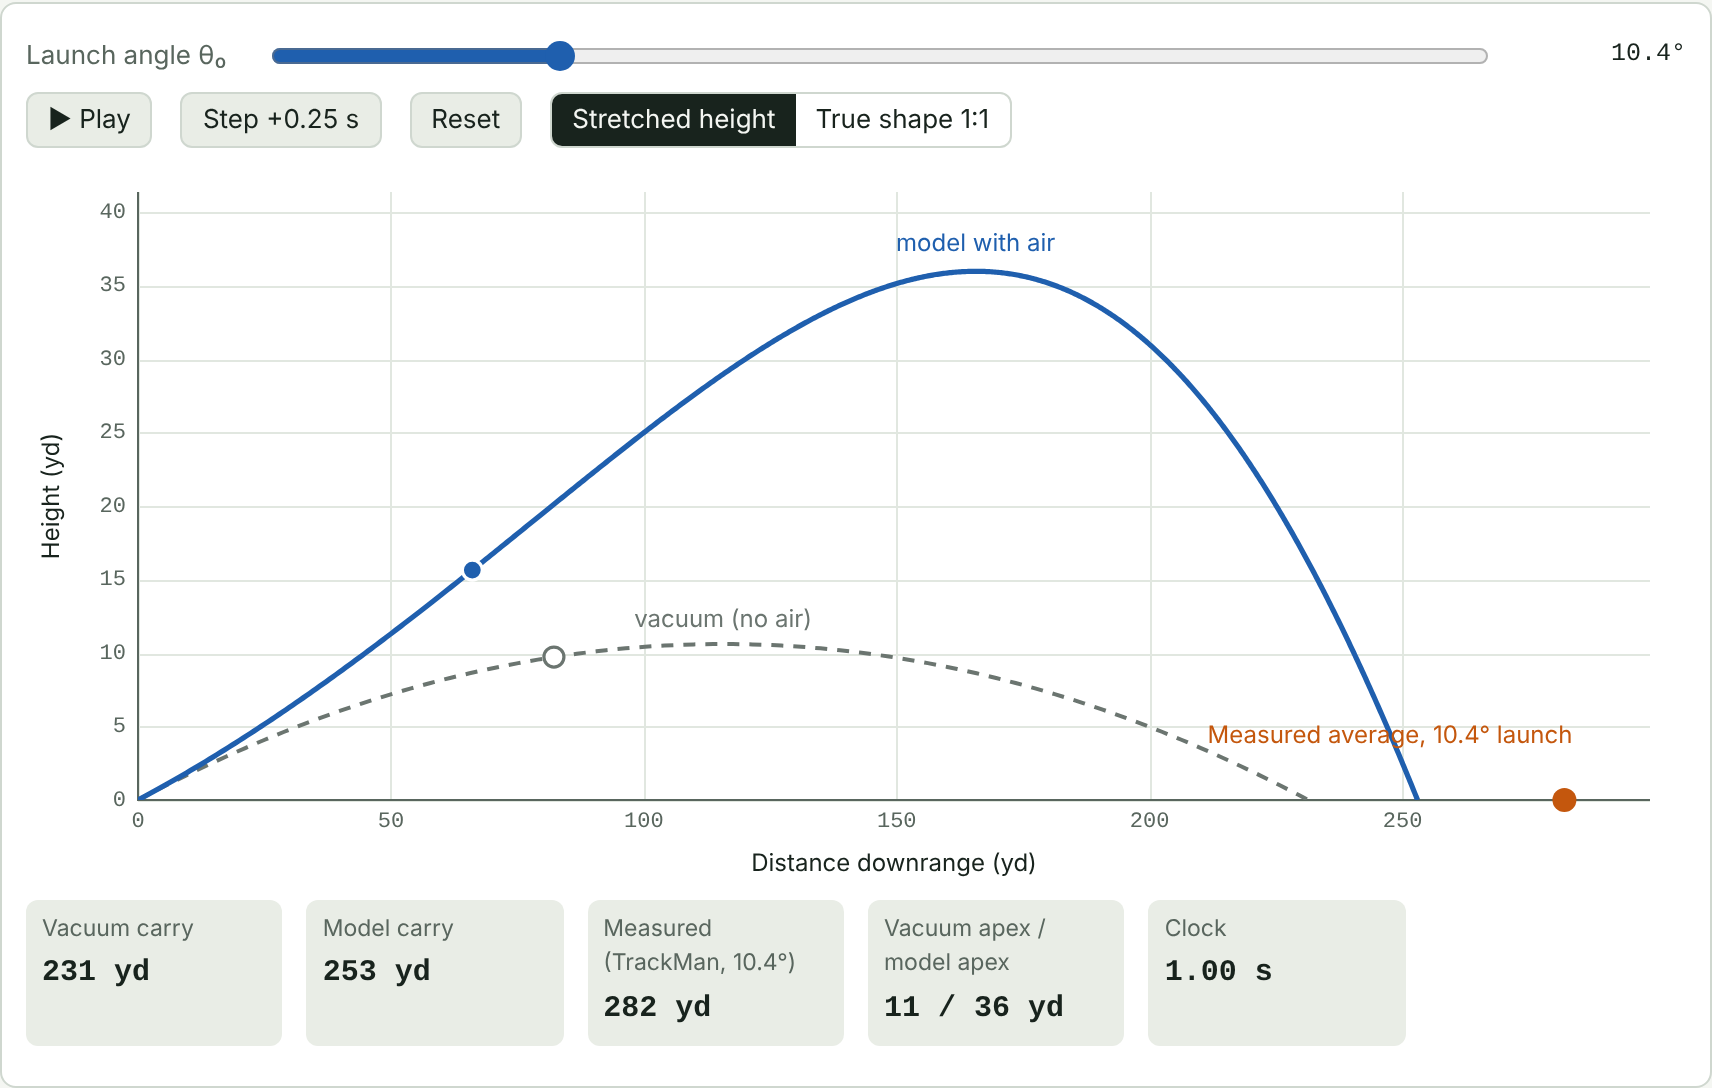
\includegraphics[width=\linewidth]{v1.png}\end{minipage}\hfill
\begin{minipage}[t]{0.49\linewidth}\centering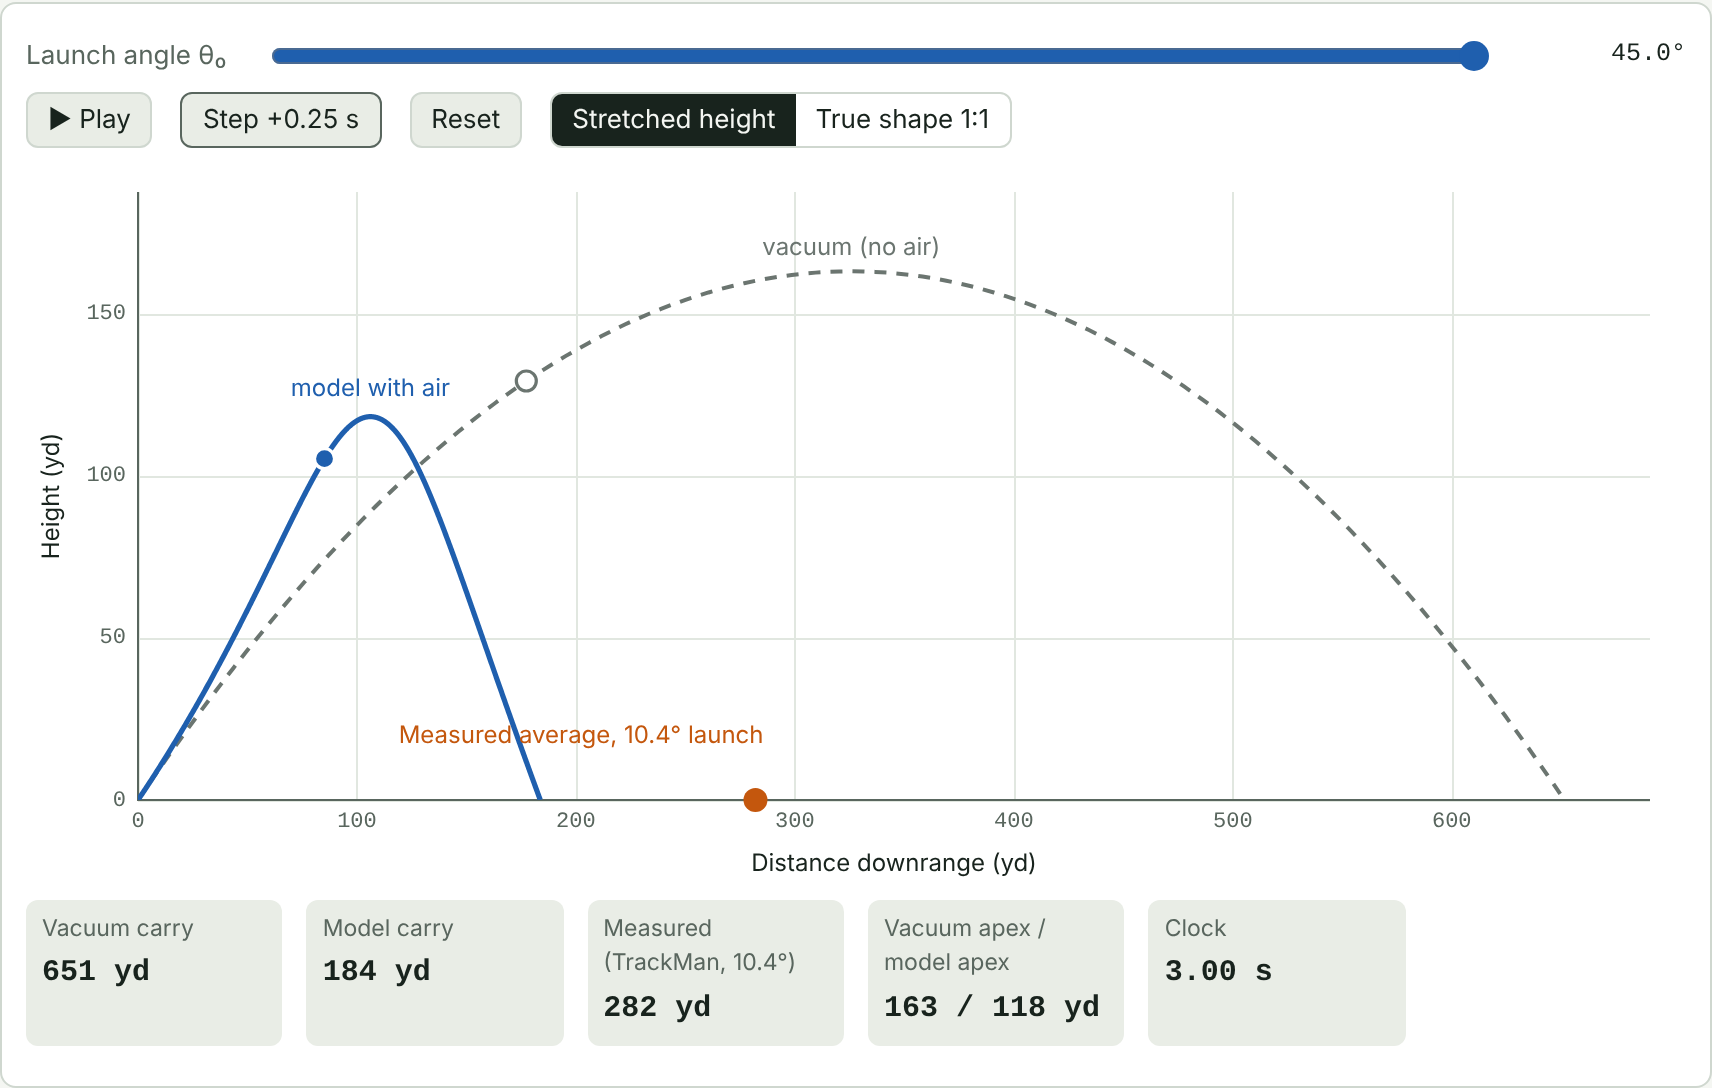
\includegraphics[width=\linewidth]{v1_45.png}\end{minipage}
\caption{View 1. Left: at the PGA driver's measured launch angle (\ang{10.4}), vacuum (dashed),
model (blue) and measured average carry (orange). Right: the same slider at \ang{45}, where the vacuum
ball flies far beyond the ball in air.}\label{fig:v1}\label{fig:v1b}
\end{figure}
\textbf{Question:} why does the projectile formula not match a real drive?
\textbf{Data:} $\theta_0$ (input); $v_0=\SI{171}{mph}$ and \SI{2545}{rpm} fixed at the 2023 PGA
driver averages; closed-form vacuum range; model trajectory; measured carry.
\textbf{Form:} side-view line chart with zero-based axes in one distance unit, because distance and
height are spatial and position is the most accurate encoding; a true-shape (1:1) toggle shows how
flat a real drive is. \textbf{Interaction:} the angle slider redraws both curves; play/pause and step
animate both balls in real time; hover reads $(x,z,t)$. At \ang{10.4} the model carries
\RawDrvCarry{}~yd against the vacuum's \VacDrv{}~yd; at \ang{45} the order flips
(\VacDrvFortyFive{}~yd vacuum vs.\ \ModDrvFortyFive{}~yd model).
\textbf{Connection:} raises ``which forces are missing?'', answered in View~2.

\subsubsection*{View 2 --- Three forces (middle: mechanism)}
\viewfig{v2.png}{View 2: free-body vectors on a true-shape path (one shared scale in newtons) and
force magnitudes over time, with the shared time cursor.}{fig:v2}
\textbf{Question:} which forces act and how do they change? \textbf{Data:} $mg$, $F_D$, $F_L$ and the
velocity direction from the current shot's trajectory. \textbf{Form:} vectors show direction; the
linked force--time chart shows magnitude precisely. The path is drawn at true shape so the arrows'
angles are physical. \textbf{Interaction:} time slider, play/pause, step, or click the chart; hover
reads the forces. At launch lift is \WFL{}~N against a weight of \Wweight{}~N, so the ball climbs.
\textbf{Connection:} the forces depend on $C_D$ and $C_L$, which View~3 explains.

\subsubsection*{View 3 --- Where lift and drag come from (middle: mechanism)}
\viewfig{v3.png}{View 3: $C_D$ and $C_L$ against spin ratio, the fitted range shaded, and the
current shot's state; right, a qualitative Magnus sketch (labeled as such).}{fig:v3}
\textbf{Question:} why does spin make lift, and why do dimples matter? \textbf{Data:} Eq.~(2) evaluated
at the current shot's Reynolds number, plus dashed curves at Re = 70k, 140k, 210k.
\textbf{Form:} line chart of two continuous quantities; the blue marker traces the shot through
coefficient space as $S$ rises during flight. \textbf{Interaction:} shares View~2's clock; hover gives
exact coefficients; the dimpled/smooth toggle substitutes a smooth-sphere $C_D=0.5$ and reports the
carry (\RawDrvCarry{}~yd dimpled vs.\ \SmoothCarry{}~yd smooth for the PGA driver).
\textbf{Connection:} with the mechanism in hand, View~4 hands over control.

\subsubsection*{View 4 --- Launch explorer (middle: exploration)}
\viewfig{v4.png}{View 4 with three pinned shots (PGA driver, 7-iron, PW, each loaded from its
measured averages) and the PGA measured carries as orange ground markers.}{fig:v4}
\textbf{Question:} how do speed, angle, and spin trade off? \textbf{Data:} $v_0,\theta_0,\omega_0,\alpha$
in; carry, apex, time, landing angle, lateral out; TrackMan markers. \textbf{Form:} side-view
trajectory (height axis labeled ``stretched'') with a numeric readout and a validity badge.
\textbf{Interaction:} sliders recompute live in the browser; ``Load measured club'' fills the sliders
from the data; pin up to three shots; hover reads $(x,z,t,u,S)$. \textbf{Connection:} the current shot
drives Views 2, 3, 5, 6, 7.

\subsubsection*{View 5 --- The optimal launch window (middle: exploration)}
\viewfig{v5.png}{View 5 at \SI{171}{mph}: carry over launch angle and spin, contours every
\SI{10}{yd}, hatching where more than half the flight is extrapolated, the measured PGA driver, and
the map's maximum.}{fig:v5}
\textbf{Question:} at a given ball speed, which angle--spin combination carries farthest?
\textbf{Data:} precomputed $61\times61$ grids. \textbf{Form:} heat map with a sequential single-hue
scale (ordered magnitude) plus contour lines, which give an accurate read where color is weak.
\textbf{Interaction:} speed slider (the optimum marker animates to its new position), tour filter,
hatching toggle, hover for exact carry, click a cell to load it into View~4. At \SI{171}{mph} the
map's best carry is \OptCarry{}~yd at \ang{\OptTheta} and \OptRpm{}~rpm.
\textbf{Connection:} View~6 asks how the environment moves the result.

\subsubsection*{View 6 --- Wind, altitude, and curve in 3D (middle: exploration)}
\viewfig{v6.png}{View 6: scenario A (sea level, calm) against the current shot (Denver altitude, 10
mph headwind, \ang{8} axis tilt), with top and side insets and $\Delta$carry readouts.}{fig:v6}
\textbf{Question:} how do wind, air density, and a tilted spin axis change where the ball lands?
\textbf{Form:} 3D is justified here because a tilted axis produces sideways lift; because perspective
distorts length, exact values come from the two orthographic insets and the readout.
\textbf{Interaction:} wind, altitude, and tilt sliders; play/pause and step; drag to orbit, wheel to
zoom, camera presets; save scenarios A and B for overlay and $\Delta$carry. \textbf{Connection:} ends
exploration and asks how far to trust the model.

\subsubsection*{View 7 --- Model vs.\ measurement (ending)}
\viewfig{v7.png}{View 7: model against TrackMan carry for all 23 clubs (equal, zero-anchored axes;
filled = mostly inside the fitted range), and the current shot's carry under vacuum, drag-only, and
full models.}{fig:v7}
\textbf{Question:} how close is the model, and which force matters most? \textbf{Form:} scatter with a
$y=x$ reference on equal zero-anchored axes so deviations are not exaggerated; bars start at zero.
\textbf{Interaction:} metric (carry, apex, landing angle), tour filter, coefficient set, hover, click
to load a club. The full per-club table is reproduced in Table~\ref{tab:val}. Below the charts the page
lists the evidence-backed insights and limitations (Section~\ref{sec:concl}).

\paragraph{Honest encoding.} Every axis names its quantity and unit, and the unit toggle changes
labels and values together. Measured is always orange and model always blue. Bars start at zero,
the validation scatter uses equal zero-anchored axes, and Views~1--2 offer or use true shape. Heat-map
color is sequential and single-hue with its range stated. Qualitative elements (the Magnus sketch, the
smooth-sphere comparison) are labeled. Light and dark themes are both supported.

\subsection{Construction}\label{sec:launch}

\begin{itemize}
\item \texttt{js/physics.js}: the model (RK4, coefficients, atmosphere); runs in the browser and in
Node, which is how it is cross-checked against \texttt{prep/model.py}.
\item \texttt{js/charts.js}: a small Canvas plotting helper (linear scales, nice ticks, tooltips,
marching-squares contours, sequential color ramp).
\item \texttt{js/core.js}: shared state (current shot, environment, coefficient set, units),
events, sliders, and the animation clock. \texttt{js/v1\_vacuum.js} \ldots{} \texttt{js/v7\_validation.js}:
one file per view. \texttt{js/main.js}: top bar, computed insights, and Methods section.
\end{itemize}

\noindent\textbf{Launch.} Unzip and double-click \texttt{index.html}; no server, internet, or
installation is needed. To deploy on obi2, copy the folder to \texttt{\textasciitilde/public\_html/golf/}.
To rebuild all data from the raw CSV (Python 3.10+ with numpy and pandas; Node.js for check N3):
\begin{lstlisting}[language=bash]
python3 prep/prepare.py && python3 prep/grid.py && python3 prep/checks.py \
  && python3 prep/bundle.py && python3 prep/report_numbers.py
\end{lstlisting}

% =====================================================================
\section{Timeline and Evaluation}

\paragraph{Timeline.} Proposal submitted and approved \todo{(date)}; model, data pipeline, and checks
built and passing; seven views implemented and revised after review (Section~\ref{sec:rev});
peer feedback \todo{(date)}; live presentation \todo{(date)}.

\subsection{Numerical and boundary checks}

All checks are run by \texttt{prep/checks.py}; \NPass{} of \NChecks{} pass (Table~\ref{tab:checks}).

{\footnotesize
\begin{longtable}{@{}p{0.04\textwidth}p{0.26\textwidth}p{0.17\textwidth}p{0.38\textwidth}p{0.06\textwidth}@{}}
\caption{Verification results (generated from \texttt{data/checks.json}).}\label{tab:checks}\\
\toprule ID & Check & Expected & Observed & Result \\ \midrule \endfirsthead
\toprule ID & Check & Expected & Observed & Result \\ \midrule \endhead
\inputrows{checks_table.tex}
\bottomrule
\end{longtable}}

\paragraph{Worked numerical example (N5).} For the PGA driver at launch,
$v_0=171\times0.44704=\SI{76.44}{m/s}$ and $\omega_0=2545\times2\pi/60=\SI{266.5}{rad/s}$, so
$S_0=0.021335\times266.5/76.44=\WSzero$ and $\mathrm{Re}_0=1.225\times76.44\times0.04267/1.81\times10^{-5}=\WRe$.
Then $C_D=0.24+0.18(\WSzero)+0.06\sin\{\pi(\WRe-\num{90000})/\num{200000}\}=\WCDzero$ and
$C_L=0.54(\WSzero)^{0.4}=\WCLzero$. With $\tfrac12\rho A u^2 = \tfrac12(1.225)(\SI{1.430e-3}{m^2})(76.44)^2$,
drag is $F_D=\WFD$~N and lift $F_L=\WFL$~N, against a weight of \Wweight~N. The model's
recorded state at $t=0$ matches the hand calculation to $10^{-9}$.

\paragraph{Boundary case that caught a bug (B3).} On the first run, a flat launch
($\theta_0=0$, no spin) never ``landed'': the landing test skipped the first step and then required
the previous height to be non-negative, which it never was again, so the shot ran to the
\SI{20}{s} limit and returned no carry. The guard was removed in both the JavaScript and Python models,
the validation runs and View~5 grids were recomputed with the fixed code, and the check now passes
(carry \SI{0}{yd}: a ball launched flat from ground level with too little lift lands at once).

\subsection{Validation against TrackMan}

{\small\begin{longtable}{@{}llrrrrrrrr@{}}
\caption{Per-club validation (generated from the \texttt{validation} SQL view). Raw = Smits and
Smith wind-tunnel constants; Cal.\ = calibrated to the PGA driver ($C_{d1}=\CalCdOne$,
$C_{l1}=\CalClOne$). Last column: \% of flight outside the fitted range.}\label{tab:val}\\
\toprule
 & & \multicolumn{1}{c}{Meas.} & \multicolumn{2}{c}{Raw} & \multicolumn{2}{c}{Cal.} & Apex (yd) & Land (\textdegree) & Out \\
Tour & Club & carry & model & err & model & err & meas/model & meas/model & \% \\
\midrule \endfirsthead
\toprule Tour & Club & Meas. & Raw & err & Cal. & err & Apex & Land & Out\\ \midrule \endhead
\inputrows{validation_table.tex}
\bottomrule
\end{longtable}}

\noindent Mean absolute carry error with the wind-tunnel constants is \MaeRawP{}~yd (PGA) and
\MaeRawL{}~yd (LPGA); with calibrated constants it is \MaeCalP{}~yd and \MaeCalL{}~yd. Apex is
reproduced to within \MaeApexRawP{}~yd (PGA) and \MaeApexRawL{}~yd (LPGA) on average, and landing
angle to within \MaeLandRawP\textdegree{} and \MaeLandRawL\textdegree.

\subsection{Feedback and revisions}\label{sec:rev}

\paragraph{Self-review revisions (from rendering every view and reading every number).}
\begin{enumerate}
\item The heat map's full-range color scale made almost every cell the same dark blue; the scale now
covers the top \SI{60}{yd} and says so.
\item Drag was drawn in the same orange as measured data, breaking the color rule; drag is now violet.
\item The spin slider's 25-rpm step displayed 2545~rpm as 2550; the step is now 1~rpm.
\item The drag-coefficient readout in View~3 showed ``NaN'' because two constants were not merged into
its parameters; fixed.
\item Labels overlapped curves and markers in Views 1, 3, 5, and 7; repositioned, and the View~5
labels drawn with a contrasting outline.
\item Force arrows in View~2 were too short to read once the ball slowed; the shared scale was
enlarged and the path redrawn at true shape so arrow angles are real.
\item The 3D view's first camera looked straight down the target line, hiding the curve; it now
opens at an angle, with presets for behind, side, and top.
\end{enumerate}

\paragraph{Peer feedback.} \todo{Before the presentation, ask three to five classmates to try three
tasks (for example: ``find the launch angle that maximizes carry at 150 mph'', ``explain why a
headwind hurts more than a tailwind helps'', ``which clubs does the model fit worst, and why?'').
Record who tried it, what they found confusing, and what you changed, in a short table here.}

% =====================================================================
\section{Contingency and Collaboration}

\begin{table}[H]\centering\small
\begin{tabularx}{\linewidth}{@{}X X@{}}
\toprule
Risk & Response \\
\midrule
Network or CDN failure during the live demo. & Avoided by design: no external dependencies; the page
runs offline from \texttt{index.html}. A second copy is on obi2. \\
Coefficient model fits irons poorly. & Realized. Irons are labeled as extrapolated in every view and
the validation reports the gap instead of tuning it away. \\
Calibration cannot meet $\pm5\%$ inside the paper's ranges. & Not realized: \CalErrPct\% (but at the
edge of the allowed range, which is reported). \\
3D too slow or confusing. & Not realized; the insets and readouts remain the exact read-out, so the
view works even if the 3D panel is ignored. \\
Schedule slip. & All seven views are complete; six remain even if one is cut. \\
\bottomrule
\end{tabularx}
\end{table}

\noindent\textbf{Collaboration and roles.} Individual project. I am responsible for the physics model,
data transcription and preparation, implementation, testing, writing, and the presentation.
Classmates contributed only as usability testers.

% =====================================================================
\section{Conclusion}\label{sec:concl}

The story answers its question with evidence rather than assertion. These insights are supported by
the model and data in the working artifact:
\begin{itemize}
\item \textbf{Air is not just a brake.} At the PGA driver's measured launch, a vacuum ball carries
\VacDrv{}~yd, the model \RawDrvCarry{}~yd, and the tour average 282~yd. Drag alone would cut the
carry to \DragOnly{}~yd; lift gives it back and more.
\item \textbf{There is an interior optimum.} At \SI{171}{mph} the best carry on the map is
\OptCarry{}~yd at \ang{\OptTheta} and \OptRpm{}~rpm. Too little spin loses lift; too much adds drag.
\item \textbf{Headwind hurts more than tailwind helps}: \HeadLoss{}~yd lost to a \SI{10}{mph}
headwind versus \TailGain{}~yd gained from an equal tailwind, because drag scales with the square of
air speed. At \SI{5280}{ft} ($\rho=\DenverRho$~kg/m$^3$) the drive carries \DenverGain{}~yd farther.
\item \textbf{The model is right where it was fitted and wrong where it was not.} It matches the
driver's apex and landing angle closely but under-predicts its carry by \RawDrvErr{}~yd; calibration
fixes the driver (\CalErrYd{}~yd) and makes the 22 held-out clubs worse (\HeldRaw{} to \HeldCal{}~yd
mean absolute error). Irons, which spend at least \IronOutside\% of their flight outside the fitted
range, land \IronLandErr\textdegree{} shallower than measured on average.
\end{itemize}

\noindent\textbf{Limitations.} The aerodynamic fit comes from one 1990s ball and is stated for
drivers only; the model is a point mass with no roll, flat ground, and uniform wind; TrackMan values
are averages over many shots, and because flight is nonlinear the carry of the average launch need
not equal the average carry; and calibration used a single target, with the best fit on the edge of
the allowed range. A natural next step would be a spin-dependent drag fit from modern-ball data for
the high-spin iron regime.

% =====================================================================
\section*{Disclosure of AI Assistance and Verification}
I used Claude (Anthropic) to help write and debug the JavaScript and Python code, the SQL, the
verification script, and to draft this report and the presentation slides. I verified the work as
follows: \todo{(edit to match what you actually did)} I transcribed both TrackMan tables myself and
checked them against TrackMan's own meter columns; I checked every model constant and equation
against the Smits and Smith paper (pp.~346--347); the numerical example in N5 was recomputed by hand;
the \NChecks{} automated checks compare the model with closed-form results, a halved time step, and
an independent second implementation; and I used every view and control in the browser before the
presentation. Every number in this report is generated from the project's data files. All design
decisions and the final text are my responsibility.

% =====================================================================
\begin{thebibliography}{99}\small
\bibitem{bearman1976} P.~W. Bearman and J.~K. Harvey, ``Golf ball aerodynamics,''
\emph{Aeronautical Quarterly}, vol.~27, no.~2, pp.~112--122, 1976.
\bibitem{choi2006} J.~Choi, W.-P. Jeon, and H.~Choi, ``Mechanism of drag reduction by dimples on a
sphere,'' \emph{Physics of Fluids}, vol.~18, 041702, 2006.
\bibitem{llmstory} Y.~Kumar, ``The LLM Story Revised with NO Human-In-The-Loop'' (course exemplar),
video, YouTube. \url{https://www.youtube.com/watch?v=PHBoa0n2Pgs}
\bibitem{munzner2014} T.~Munzner, \emph{Visualization Analysis and Design}. Boca Raton, FL: CRC
Press, 2014.
\bibitem{penner2003} A.~R. Penner, ``The physics of golf,'' \emph{Reports on Progress in Physics},
vol.~66, no.~2, pp.~131--171, 2003.
\bibitem{phet} PhET Interactive Simulations, ``Projectile Motion,'' University of Colorado Boulder.
\url{https://phet.colorado.edu/en/simulations/projectile-motion}
\bibitem{smits1994} A.~J. Smits and D.~R. Smith, ``A new aerodynamic model of a golf ball in
flight,'' in \emph{Science and Golf II: Proceedings of the World Scientific Congress of Golf},
A.~J. Cochran and M.~R. Farrally, Eds. London: E \& FN Spon, 1994, pp.~340--347.
\bibitem{trackman2023} TrackMan, ``Introducing updated Tour averages'' (2023 PGA Tour and LPGA Tour
averages tables). \url{https://www.trackman.com/blog/introducing-updated-tour-averages}
\bibitem{ussa1976} NOAA, NASA, and USAF, \emph{U.S. Standard Atmosphere, 1976}. Washington, DC: U.S.
Government Printing Office, 1976.
\bibitem{victor2011} B.~Victor, ``Explorable Explanations,'' 2011.
\url{http://worrydream.com/ExplorableExplanations/}
\end{thebibliography}
\end{document}
